%%%%%%%%%%%%%%%%%%%%%%%%%%%%%%%%%%%%%%%%%%%%%%%
\chapter{How Might Online Systems Support Citizen-led Knowledge Work}

\begin{quote}
\emph{This dissertation explores how }
\end{quote}
\vspace{0.25in}

Todo- text here

\section{Opportunity: Harnessing humanity\textquotesingle s collective efforts accomplishes great goals}
Luis von Ahn said people can build eiffel towers but people are barely able to build those eiffel towers - -why? But why build eiffel towers for other people?

poor signal-to-noise from crowds due to lack of training; inefficient collaboration without careful attention; and poor results (or no results at all) unless experts lead. To address these concerns, my work introduces and evaluates peer production architectures and procedural learning.

\subsection{People have complementary knowledge in comparison to experts and are uninfected by expert biases}
--drawn from lived experience
-- individually and collectively

Sometimes, having a different background than experts can
be beneficial. Shared knowledge is great when it’s right, but
blocks progress when wrong. When false assumptions limit
experts, at least some novices are likely to be “uninfected”.
For example, GalaxyZoo volunteers discovered ‘green pea’
galaxies overlooked by scientists who mistakenly assumed
the green hue was merely an imaging artifact [54]. 

\subsection{Learning resources proliferate and people learn from personal interest/hobby but it's not directly linked to their personal thing}
Creative, open-ended work has rich pedagogical value.
Online work, like online learning, requires appropriate
scaffoldings, such as rubrics [12,41], decision trees [43,57],
tutorials [6], and quick expert guidance [23]. Similar to
general critique of pure discovery learning [47], simply
asking participants to “figure it out” would be poor pedagogy. Hence, Gut Instinct introduces a guided discovery
learning approach as Mayer advocates: expert-curated
learning materials help participants start, with discovery
following. Recruiting learners as citizen scientists offers a
Problem-based Learning experience with context and motivation for the material students learn [50]. In principle,
these real-world problems also provide a yardstick for
measuring learning. 

\subsection{Second-order effect: People are connected online and collectively have access to many resources}
In a large distributed community, there’s often
someone who happens to have important relevant
knowledge, usually drawing on a relevant but distant domain. Such distributed efforts are a type of lead-user innovation [31]. Having many people work on the same problem increases the odds that one will break through. Drawing
on secondary expertise as inspiration can be an important
agent of creativity because almost by definition, the combination is rare [10]. Open \& crowd innovation builds up on
contributions by diverse online participants, and a ‘bubbling
up’ process for strong ideas [56].

\section{Challenge: People don't know how to perform expert work}
Problem Dimensions


\subsection{People lack the expertise to make situationally-appropriate choices and people aren\textquotesingle t trained in these things}
-- people dont know how to use their knowledge
Why is this complex: requires making many choices

The
converse also holds, and much more often: novices are also
“uninfected” by all the knowledge that enables experts to
innovate.

\subsection{People lack a professional network to improve their work}


\subsection{People lack the time/remuneration/resources to learn new things and implement them in their lives}
nnk

********
Further, recreating expert work context, process, and outcomes can alter and reduce the value of novice contributions.

My research raises the question: how can global communities create knowledge that meets their goals without waiting for experts to lead? My research prototypes collective systems for large-scale problems.

********
\section{Thesis: Procedural Support for Roles}

Many people have strong personal motivations and contextual insights. To create knowledge,
they need mental scaffolds for organizing complex work, domain knowledge to compose and
execute the steps, and ways to ask for help. Professional scientists benefit from conceptual
knowledge, professional training, pre-existing organizational structure for collaboration, and direct access to resources. Currently, citizens lack these resources.

Building on these new participation channels, we suggest that democratizing experimentation may
also expand the gamut of scientific knowledge. People have questions about their health, but lack
the expertise and resources to scientifically investigate them. How might online systems support
more complex activities that leverage the creativity and diversity of a global community?

This dissertation explores challenges people face xxxxxxx. Underlying these investigations is the thesis:

//this is where you introduce the taxonomy 

"My thesis statement is"
\begin{quote}
\emph{Understanding how the tension between exploring data and explaining process manifests itself in practice makes it possible to design software that enables analysts to document and share their work more effectively.}
\end{quote}




\section{Contributions}
This dissertation has four types of contributions: empirical results, theoretical perspectives, prototype systems, and an open dataset. Here I summarize these contributions in the order they will be presented in the chapters that follow (Figure \ref{fig:contributions}).

"This dissertation makes contributions in a number of areas.

\subsection{Theoretical: Techniques and Framework}
\begin{itemize}
\item procedural learning helps -- docent and galileo experiments
\item Roles Support via Just-in-time Skill Acquisition
 People take different roles
\item  Systems that divide the task between people, community, and machines
-- Principles to Integrate Learning in Social Computing
	1) deeper work — more learning   //     2) more work — better collaboration

\end{itemize}

All these techniques have been put in systems

\subsection{System Design (including Interfaces)}
1. UIs that integrate learning and focused collaboration
2. 

\subsection{Empirical Results from Real-world Deployment}
expertise: limited; diversity: different countries; scale: some


\subsection{Dataset}

A Venn diagram showing the contributions and the domains

//Philosophical -- how does this research think and imagine differently; and how that was operationalized as techniques as systems
-- People have an amazing breadth and depth of ideas and work with them


\begin{figure}[t!] 
  \centering
    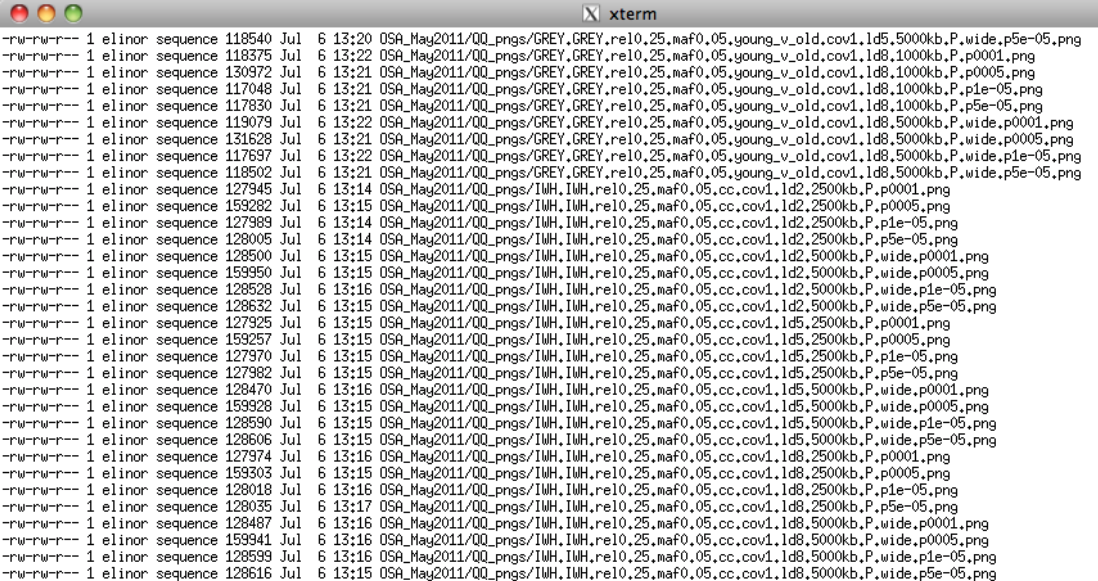
\includegraphics[width=1.0\textwidth]{img/files}
  \caption[Contributions of this dissertation]
{Contributions of this dissertation including empirical results, prototype systems, theoretical perspectives, and an open dataset.}
  \label{fig:contributions}
\end{figure}

\section{Impact}
 \subsection{Used by communities}
 \subsection{Talks in the Research community and other communities}
 \subsection{Taught in classes}


\section{Dissertation Roadmap}

%%%%%%%%%%%%%%%%%%%%%%%%%%%%%%%%%%%%%%%%%%%%%%%%%%%%%%%%%%%%%%%%%%

\chapter{Related Work}
This chapter summarizes related work in social computing, online learning, citizen science, psychology, and health that has provided useful insights to design the systems in this thesis.


we need three things
1. right sets of people
2. right architectures to co-ordinate them
3. integrating learning resources 


\begin{quote}
\emph{This dissertation explores how }

\end{quote}
\vspace{0.25in}

%%%%%%
\section{Lead Users Succeed When People Know What to Do and How to Do It}
-- Techniques and systems to build expertise in people (toolkit?)

1. GitHub: enables storing code, sharing code, great, but doesn’t teach how to program
2. Technology systems currently use existing capacity and takes away the context that they have — how do you build capacity — people have the context 
3. techniques to build expertise in people
4. difference between lead users and end users? 
5. examples: UN example (see eric vh)

\subsection{People haven't thought about lead/end users as communities}

\subsection{End users can program, write, and perform data analysis but dont know how to experiment}
-- A new domain for end-user programming 
End users as designers

contr -- exp design workflow, learning to generate a hypothesis

-- Thinking differently about hci 
  people are not just information processing machines
  people are social, have motivations and goals

1. HCI work focuses on programmers, end-user programmers, "even casual users” - individuals
2. also, these tasks are CS specific (like writing)
3. we focus on a general-purpose task (like experimentation), on novices, and on communities


%%%%%%%
\section{Online Learning Resources Emphasize Conceptual Understanding in Fake Settings Over Procedural Learning for Real Questions}

Current online learning scales the classroom.

\subsection{personally meaningful learning and doing}
-- JIT learning techniques embedded in people’s doing

%%%%%%
\section{Crowdsourcing Does Not Support Personally Meaningful Work}


\subsection{Systems and architectures for crowdsourcing complex work}


\subsection{People discuss online but don't do stuff}
//TODO1: Unclear what i'm going for here
1. Meaningful social computing systems need learning
    1. my work shows how to inject learning in social computing systems

1. What is the purpose of building social computing systems?
-- probe an idea and see how far it goes (See msb)
2 .open-ended, creative tasks
3. 1. Improve the quality of poor contributions — and improve the quality of max contributions 
    1. — hockey stick curve 
4.
    1. lowers the threshold for designing an experiment - how: procedural learning
    2. support reviewing and running an experimentation with system support


%%%%%%
\section{Specific domain: Citizen Science}
-- An expansion of the depth and breadth of work performed by citizen science communities

Internet-scale science misses people’s lived experience
Science is increasingly networked, multidisciplinary, and
open [34]. For instance, LIGO’s pathbreaking discovery of
gravitational waves brought together over 100 researchers
from over 100 institutions across 18 countries
(ligo.org/about). Scientists increasingly share data and results faster (arxiv.org). Large scientific projects, like the Human Genome Project, took to agile science by sharing
methods, data, and insights to collaboratively speed discoveries. Scientists also form global collaborations to accelerate
research in nascent scientific domains, like the Earth Microbiome project (earthmicrobiome.org).
At its best, institutional science has benefitted immensely
from large-scale global collaboration. Complementing this,
many online projects enable people to help scientists: annotating scientific papers [14]; labeling galaxies [20]; folding
protein structures [9] and providing microbiome samples
[32], CPU cycles (worldcommunitygrid.org), or personal data
(openhumans.org). However, public involvement continues
to be largely limited to performing tasks just beyond the
reach of computers. This is not without reason—a lot of scientific work requires deep conceptual knowledge and training in scientific process to perform useful work. Most
citizens lack the time, resources, and motivation to develop
narrow, unique skillsets.
In the quest to get people to track, measure, accumulate, or
sort both digital and analog data, citizen science has overlooked the massive opportunity of leveraging people’s
unique advantages: our skills as reflective, creative thinkers
who generate theories about the world, including ourselves.
People can offer more than just their data and perceptual
skills: they create theories, right or wrong, about a wide
range of topics including emotions [19], motivation [30], or
diet. These may be observational theories [22], folk theories
passed in a family/culture across generations [13], or ideas
brainstormed in online communities [1]. Perhaps, these intuitions can provide a starting point for personally meaningful
scientific work that also assists the scientific community.
Can people be scientists rather than just sensors?
Advances in precision medicine have demonstrated the need
to engage people in uncovering and sharing insights [5]. People are highly motivated to improve their health outcomes,
more so if they suffer from a condition that severely affects
their quality of life, naturally forming communities. For example, patients from the Amyotrophic Lateral Sclerosis
(ALS) community on Patients Like Me (patientslikeme.com)
organized a study to track effects of Lithium on their symptoms [45]. This is not surprising; lead users excel at tackling
need-intensive problems where they can use their lived
experiences to identify problems, try solutions, and readily
observe the effects [18]. Other organized communities like
Quantified Self hope to uncover lifestyle patterns that may
improve their productivity and health outcomes. The word
‘self’ belies the fact that such movements are highly collaborative: amateurs frequently share experiences and invite
feedback on online fora (patientslikeme.com) and blogs
(ibsgroup.org). Millions follow these ideas and some incorporate these intuitions in their lives. How can people expand
their insights into scientific work?
Most scientists develop their skills through an apprenticeship-based graduate school experience. Apprenticeships emphasize hands-on experience with individualized, taskspecific feedback [40]. Scientists possess a wealth of declarative knowledge about their domains (e.g., how to set up a
randomized controlled trial), and also procedural knowledge
—some narrow, some broad—towards getting things done
(e.g., improving fMRI signal intensity by having participants
consume cocoa beforehand [11]).This work explores how
online learning and process training systems, combined with
peer collaboration, can help people learn similar skills that
can be useful in scientific and design domains

Modern science is increasingly collaborative
[57]: citizens count bird species, identify galaxies, edit protein structures, and create novel hypotheses [16,59,73]. One reason is that different people provide different expertise that can vet
claims and fix mistakes [33]. Collaboration benefits creativity when it brings different perspectives that build on each other; it impedes creativity (or worse, causes regression) when—through
groupthink—it spreads biases rather than removing them [68]. A humbling example of the power
of fresh eyes: volunteer citizen scientists identified a new class of galaxies (“green pea” galaxies)
after researching green blots on Galaxy zoo images; experts had dismissed these images as apparatus error [6]. Such collaboration requires strategic isolation: providing just enough scaffolding
to keep biases independent, while not stifling original ideas for bottom-up knowledge creation.
While public contributions have supported institutional science; it’s rare for citizens to design
their own experiments. Despite a predetermined goal and a formalized process, experimentation
requires making situationally-appropriate decisions. A dependent variable may produce crisp
numbers but feedback on the experiment design itself is more multifarious. Good experiment
design is inherently user centered: how will participants interpret the instructions? Experiment
designers need awareness of others’ interpretation of their ideas and asks. Feedback and iteration
might be key to creative success, especially for novices. Feedback can be provided by experts
[20,64], peers [5,40], software [19,28], or even oneself [5,64]. While feedback from novices can
potentially improve both structure and content, it can also emphasize superficial issues over the
underlying structure [11].


science is nascent, highly contextual, and personally motivating.
1. Internet-scale science misses people’s lived experience \\
 “Other people’s noise is my signal” \\
2. Can people be scientists rather than just sensors? \\
 Provide a taxonomy of sorts of citizen science work
3. Scaling up science: How open is open science? \\
 open science things assume people know the science — it’s not a right assumption — providing notebooks and books does nothing // truly open science means people know how science works
4. Microbiome research: a petri dish for making scientists \\
5. link my research with more hardcore science

**
Often, when citizens participate in science, it is as “embedded sensors” that are aggregated by experts. A classic example is Audubon’s Christmas bird count, run since 1900
[7]. Online examples include reporting flower blooms in
Project Budburst [13]; recording wildlife activity [24];
identifying galaxies from satellite imagery in GalaxyZoo
[59]; and biochemistry games: finding protein structures in
Foldit [19], synthesizing RNA molecules in EteRNA [44], and aligning nucleotide sequences in Phylo [33]. At their
best, these citizen science platforms yield novel insights.
For example, Foldit players discovered protein structures
that helped scientists understand how the AIDS virus reproduces [20].


\subsection{Petri-dish: Scaling up microbime science}
Specific domain in which this has been tried about: microbiome

Understanding the human microbiome requires insights
into people’s lifestyles
The human gut microbiome is the community of microbes
(and their gene products) interacting in the human gut.
However, research has only scratched the surface of understanding the microbiome and using it to improve our wellbeing. The American Gut Project (AGP) is the world's
largest crowdfunded citizen science project [38]. AGP
participants contribute their samples for bacterial marker
gene sequencing and analysis [22]. Participants then receive
a summary of their results with all their raw data. Anonymized data is publically available. AGP seeks to build a
comprehensive map of the human microbiome, and identify
its healthy and unhealthy components.
People hold the key to understanding the gut microbiome
The structure of the human microbiome is influenced by
many factors, including age, genetics, diet, and xenobiotic
and antibiotic use [27]. The gut microbiome in particular
plays an important role in metabolism and immune system
development, and some microbiome dysbioses have been
associated with diseases such as obesity, inflammatory
bowel disease, type I and type II diabetes, autism, multiple
sclerosis, and malnutrition [16]. The human microbiome is
impossible to understand without information about its host
[22] and many influence factors remain unknown. Teaching
people about the gut microbiome and having them guess
associations between the microbiome and health and disease states can potentially accelerate the process of discovering links between diet, disease, and lifestyle factors and
the gut microbiome.






